\section{Pseudorandom Functions}
In this section, we first define pseudorandom functions, and then show how to  construct a pseudorandom function from a pseudorandom generator.

Considering the set of all functions $f: \{0, 1\}^n \rightarrow \{0, 1\}^n$, there are $(2^n)^{2^n}$ of them.
To describe a random function in this set we need $n \cdot 2^n$ bits.
Intuitively, a pseudorandom function is one that cannot be distinguished from a random one,
but needs much fewer bits (e.g., polynomial in $n$) to be described.
Note that we restrict the distinguisher to only being allowed to ask the function poly($n$) times and decide whether it is random or pseudorandom.

\subsection{Definitions}

\begin{definition}[Function Ensemble]
    A \emph{function ensemble} is a sequence of random variables $F_1, F_2, \cdots, F_n, \cdots$ denoted as $\{F_n\}_{n \in \mathbb{N}}$ such that
    $F_n$ assumes values in the set of functions mapping $n$-bit input to $n$-bit output.
\end{definition}
Although we will only focus on the functions where the input and output bit-length is the same, the definition can be generalized to functions mapping $n$-bit inputs to $m$-bit outputs as $\{F_{n, m}\}_{n, m \in \mathbb{N}}$.

\begin{definition}[Random Function Ensemble]
    We denote a random function ensemble by $\{R_n\}_{n \in \mathbb{N}}$.
\end{definition}
A sampling of the random variable $R_n$ requires $n \cdot 2^n$ bits to describe.

\begin{definition}[Efficiently Computable Function Ensemble]
    A function ensemble is called \emph{efficiently computable} if
    \begin{enumerate}[label=(\alph*)]
        \item \textbf{Succinct}:
              $\exists$ a PPT algorithm $I$ and a mapping $\phi$ from strings to functions such that
              $\phi(I(1^n))$ and $F_n$ are identically distributed.
              Note that we can view the output of $I(\cdot)$ as the description of the function.
        \item \textbf{Efficient}:
              $\exists$ a poly-time machine $V$ such that
              $V(i, x) = f_i(x)$ for every $x \in \{0, 1\}^n$, where $i$ is in the range of $I(1^n)$, and $f_i = \phi(i)$.
    \end{enumerate}
\end{definition}

Note that the succinctness condition implies that a sample from $F_n$ can be equivalently generated by first sampling a random string $k$ from $\{0, 1\}^n$, and then outputting $f_k$. Here $k$ is often called the ``key'' of the function\footnote{An efficiently computable function requires only $n$ bits (the key) to describe, while a random function requires $n.2^n$ bits.}. More generally, the key can be a string of length $m$ where $n$ is polynomial in $m$; here $I$ uses a random tape of length $m$ and outputs $n$ bits. %However, we will only consider the case where the key is of length $n$.

\begin{definition}[Pseudorandom Function Ensemble]
    A function ensemble $F = \{F_n\}_{n \in \mathbb{N}}$ is \emph{pseudorandom} if
    for every non-uniform PPT oracle adversary $\ma$, there exists a negligible function $\epsilon(n)$ such that
    \[
        \big| \Pr[\ma^{F_n} (1^n) = 1] - \Pr[\ma^{R_n} (1^n) = 1]  \big| \leq \epsilon(n).
    \]
    Here by saying ``oracle'' it means that $\ma$ has ``oracle access'' to a (fixed) function (in our definition, the function is a sampling of $F_n$ or $R_n$), and each call to that function costs 1 unit of time.
\end{definition}

Note that we will only consider efficiently computable pseudorandom ensembles in the following. Therefore, each function in $F_n$ is defined by a PRF key $k \in \{0, 1\}^n$.


\subsection{Construction of PRF from PRG}

\begin{construction}
    Given a PRG $G: \{0, 1\}^n \rightarrow \{0, 1\}^{2n}$,
    let $G_0(x)$ be the first $n$ bits of $G(x)$, $G_1(x)$ be the last $n$ bits of $G(x)$.
    We construct $F^{(K)}: \{0, 1\}^n \rightarrow \{0, 1\}^n$ as follows.
    \[
        F^{(K)}_n(x_1 x_2 \cdots x_n) := G_{x_n}(G_{x_{n-1}} (\cdots(G_{x_1}(K)) \cdots  )),
    \]
    where $K \in \{0,1\}^n$ is the key to the pseudorandom function. In Figure \ref{fig:binary-tree}, $i = K$.
\end{construction}
The construction can be viewed as a binary tree of depth $n$, as shown in Figure \ref{fig:binary-tree}\footnote{Algorithmically, $F_n^{(K)}(x)$ is computed as:
\begin{enumerate}
    \item Set $y \gets K \in \{0, 1\}^n$.
    \item For $i = 1 \dots n$: update $y \gets G_{x_i}(y)$.
    \item Output $y$.
\end{enumerate}
}.

\begin{marginfigure}
    \centering
    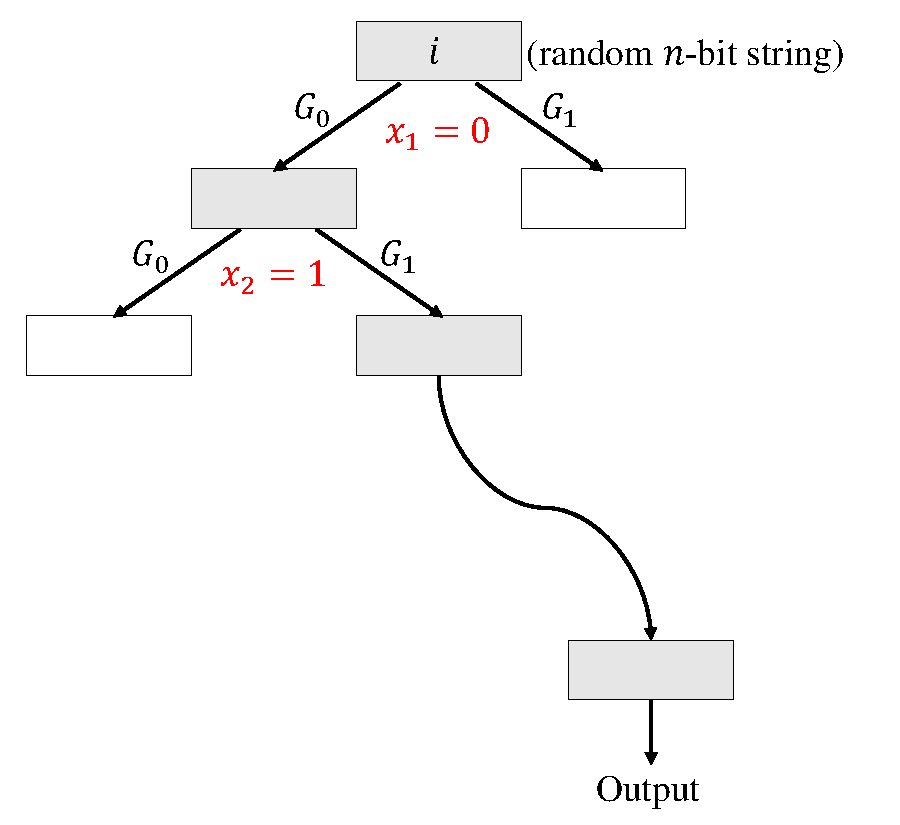
\includegraphics[width=\textwidth]{Old Scribe Notes/binary-tree.pdf}
    \caption{View the construction as a binary tree}
    \label{fig:binary-tree}
\end{marginfigure}

\begin{theorem}\label{theorem:ggm}
    The function ensemble $\{F_n\}_{n \in \mathbb{N}}$ constructed above is pseudorandom.
\end{theorem}

\proof
Assume for the sake of contradiction that $\{F_n\}_{n \in \mathbb{N}}$ is not a PRF.
Then there exists a non-uniform PPT oracle adversary $\ma$ that can distinguish $\{F_n\}_{n \in \mathbb{N}}$ from $\{R_n\}_{n \in \mathbb{N}}$. Below, via a hybrid argument, we prove that this contradicts the fact that $G$ is a PRG; we will construct an adversary $\mathcal{B}$ that can distinguish between a sample from $U_{2n}$ and $G(U_{n})$. We will prove for a fixed $n$, and the proof can be easily extended to all $n \in \mathbb{N}$.\smallskip

\noindent \textbf{Hybrids}. Consider the sequence of hybrids $H_i$ for $i \in \{ 0, 1, \cdots, n\}$ where the hybrid $i$ is defined as follows:
\[H_{i}^{(K_i)} (x_1x_2\ldots x_n ):= G_{x_n}(G_{x_{n-1}} (\cdots(G_{x_{i+1}}(K_i(x_1\dots x_{i-1}x_i))) \cdots  )), \]
where $K_i$ is a random function from $\{0,1\}^{i}$ to $\{0,1\}^n$. Intuitively, hybrid $H_i$ corresponds to a binary tree of depth $n$ where the nodes of levels $0$ to $i$ correspond to random values and the nodes at levels $i+1$ to $n$ correspond to pseudorandom values. By inspection, observe that hybrids $H_0$ and $H_n$ are identical to a pseudorandom function and a random function, respectively. Note that we cannot yet reduce the computational indistinguishability of $H_i$ and $H_{i+1}$ to security of the PRG $G$ because the adversary can make multiple oracle queries at different inputs.\smallskip

\noindent \textbf{Sub-hybrids}. We show that $H_{i}$ and $H_{i+1}$ are indistinguishable by considering a sequence of sub-hybrids $H_{i,j}$ for $j \in \{0,\ldots q\}$, where $q$ is the number of oracle queries made by $\mathcal{A}$\footnote{Observe that $\mathcal{A}$ can make at most polynomial in $n$ oracle queries. Looking ahead, our outer adversary $\mathcal{B}$ can either take $q$ as the max queries allowed to $\mathcal{A}$, or guess the number, and double the guess each time if it's an under-estimate.}.
Intuitively, with each sub-hybrid $H_{i,j}$, at level $i+1$ in the tree, we will fix the first $j$ oracle queries made by $\mathcal{A}$ to be output of random functions and the rest to be output of PRG. Let $R_i: \{0, 1\}^i \to \{0, 1\}^n$ and $S_{i}: \{0, 1\}^{i+1} \to \{0, 1\}^n$ be two random functions.
We define sub-hybrid $H_{i,j}^{(R_i, S_{i})}(x_1x_2\dots x_n)$ algorithmically as follows:
\begin{enumerate}
    \item Initialize a list $L \gets \{\}$ to store the $i$-bit prefixes of the queries made by $\mathcal{A}$.
    \item If $|L| < j$ or $(x_1\dots x_i) \in L$\footnote{Captures the first $j$ queries or any query with repeated $i$-bit prefix to a previous query.}:
          \begin{enumerate}[noitemsep,nolistsep]
              \item Set $y \gets S_i(x_1\dots x_i x_{i+1})$.
              \item Append $(x_1\dots x_i)$ to $L$.
              \item For $a \in i+2 \dots n$: update $y \gets G_{x_a}(y)$.
          \end{enumerate}
    \item Else:
          \begin{enumerate}[noitemsep,nolistsep]
              \item Set $y \gets R_i(x_1\dots x_i)$.
              \item For $a \in i+1 \dots n$: update $y \gets G_{x_a}(y)$.
          \end{enumerate}
    \item Output $y$.
\end{enumerate}

Note that $H_{i, 0}$ is the same as $H_i$ and $H_{i, q}$ is the same as $H_{i+1}$. Since we assumed that $\mathcal{A}$ can distinguish between $H_0$ and $H_n$, by triangle inequality, there exists a $i^*, j^*$ such that it can distinguish $H_{i^*,j^*}$ and $H_{i^*,j^*+1}$. We now focus on these two sub-hybrids\footnote{Looking ahead, the outer adversary $\mathcal{B}$ can guess $i^*, j^*$; total choices are bounded by polynomial in $n$. To simplify the proof, we will assume that $\mathcal{B}$ already knows this $i^*, j^*$.}. Consider the $j^*+1$-th query made by $\mathcal{A}$ (i.e. the first query where $|L|=j$). Observe that this query cannot have the same $i$-bit prefix as any of the previous queries. Because if it did, then the output distribution of the two hybrids would be identical, and that contradicts our assumption about $\mathcal{A}$'s distinguishing power. Therefore, the $j^*+1$-th query has to be a new query, and this query is the only place where the two hybrids differ.\smallskip

\noindent \textbf{Outer adversary $\mathcal{B}$}. Now we are ready to construct our outer adversary $\mathcal{B}$ that can distinguish between $U_{2n}$ and $G(U_n)$. $\mathcal{B}^{\mathcal{A}, i^*, j^*}(1^n, z)$, where $z \in \{0, 1\}^{2n}$ ($z$ could be either from $U_{2n}$ or $G(U_n)$) and we assume the knowledge of $i^*, j^*$\footnote{As mentioned before, it can be guessed with slight loss in distinguishing advantage.}, operates as follows:
\begin{enumerate}
    \item Parse $z$ as $z_0||z_1$, where $z_0, z_1 \in \{0, 1\}^n$.
    \item For all the oracle queries from $\mathcal{A}$ except the $j^*+1$-th query, respond as $H_{i^*,j^*}$\footnote{The outer adversary $\mathcal{B}$ runs a random function in polynomial time in $n$ via lazy sampling. It generates a random output on a new input and caches responses to previous inputs.}.
    \item For the $j^*+1$-th query $(x_1\dots x_n)$, do the following:
          \begin{enumerate}
              \item Set $y \gets z_{x_{i^*+1}}$.
              \item For $a \in i^*+2 \dots n$: update $y \gets G_{x_a}(y)$.
              \item Respond with $y$.
          \end{enumerate}
    \item Output whatever $\mathcal{A}$ outputs.
\end{enumerate}

We assumed that $\mathcal{A}$ can distinguish between $H_{i^*, j^*}$ and $H_{i^*, j^*+1}$, so by contrapositive of the Sunglass Lemma, $\mathcal{B}$ can distinguish between $U_{2n}$ and $G(U_n)$. This contradicts that $G$ is a PRG.

%where $q_{i+1}$ is the number of the distinct $i-bit$ prefixes of the queries of $\mathcal{A}$.\footnote{Observe that $q_{i+1}$ for each appropriate choice of $i$ is bounded by the running time of $\mathcal{A}$. Hence, this value is bounded by a polynomial in the security parameter.}
%We define hybrid $H_{i,j}$ for $j =0$ to be same as hybrid $H_{i}$. Additionally, for $j >0$ hybrid $H_{i,j}$ is defined to be exactly the same as hybrid $H_{i,j-1}$ except the response provided to the attacker for the $j^{th}$ distinct $i-bit$ prefix query of $\mathcal{A}$. Let this prefix be $x^*_n x^*_{n-1} \ldots x^*_{i}$. Note that in hybrid $H_{i,j-1}$ the children of the node $x^*_n x^*_{n-1} \ldots x^*_{i}$ correspond to two pseudorandom values. In hybrid $H_{i,j}$ we replace these two children with random values. By careful inspection, it follows that hybrid $H_{i,q_{i+1}}$ is actually $H_{i+1}$. All we are left to prove is that hybrid $H_{i,j}$ and $H_{i,j+1}$ are indistinguishable for the appropriate choices of $j$ and we prove this below.
%Now we are ready to construct an adversary $\mathcal{B}$ that  distinguishes $U_{2n}$ from $G(U_n)$: On input $T \in\{0, 1\}^{2n}$ ($T$ could be either from $U_{2n}$ or $G(U_n)$),
%construct a full binary tree of depth $n$ that is exactly the same as $H_{i,j}$ except replacing the children of  $x^*_n x^*_{n-1} \ldots x^*_{i}$ by the value $T$.
%Observe that the only difference between $H_{i,j}$ and $H_{i,j+1}$ is that values corresponding to nodes $x_n^*\ldots x_i^* 0$ and $x_n^*\ldots x_i^* 1$ are pseudorandom or random respectively. $\mathcal{B}$ uses the value $T$ to generate these two nodes. Hence success in  distinguishing hybrids $H_{i,j}$ and $H_{i,j+1}$ provides a successful attack for $\mathcal{B}$ in violating security of the pseudorandom generator.
\qed







\section{PRFs from DDH: Naor-Reingold PRF}
We will now describe a PRF function family $F_n: \mathcal{K} \times \{0,1\}^n \rightarrow \mathbb{G}_n$ where DDH is assumed to be hard for  $\{\mathbb{G}_n\}$ and $\mathcal{K}$ is the key space.
The key for the PRF $F_n$ will be $K =  (h, u_1, \ldots u_n)$, where $u,u_0\ldots u_n$ are sampled uniformly from $|\mathbb{G}_n|$, $g$ is the generator of $\mathbb{G}_n$ and $h = g^u$. Compared to the previous construction (Theorem~\ref{theorem:ggm}), there are two differences to note already: the key is polynomially longer and the output space is $\mathbb{G}_n$ instead of $\{0, 1\}^n$.

\[F_n(K,x) = h^{\prod_{i} u_i^{x_i}}\]

Next, we will prove that the function $F_n$ is a pseudo-random function or that $\{F_n\}$ is a pseudo-random function ensemble.\footnote{Here, we require that adversary distinguish the function $F_n$ from a random function from $\{0,1\}^n$ to $\mathbb{G}_n$. Note that the output range of the function is $\mathbb{G}_n$. Moreover, note that the distribution of random group elements in $\mathbb{G}_n$ might actually be far from uniformly random strings.}
\begin{lemma}
    Assuming the DDH Assumption (see Definition~\ref{def:ddh}) for $\{\mathbb{G}_n\}$ is hard, we have that $\{F_n\}$ is a pseudorandom function ensemble.
\end{lemma}
\begin{proof}
    The proof of this lemma is similar to the proof of Theorem~\ref{theorem:ggm} except for some subtle differences that arise from number theory\footnote{At a high-level, we can no longer fix nodes in the same level of the tree arbitrarily. Fixing one node has implications for how other nodes will be changed. This is because we have a fixed basis in the key.}.

    Let $R_n$ be random function from $\{0,1\}^n \rightarrow \mathbb{G}_n$. Then we want to prove that for all non-uniform PPT adversaries $\mathcal{A}$ we have that:
    \[\mu(n) = \left|\Pr[\mathcal{A}^{F_n}(1^n) =1] -  \Pr[\mathcal{A}^{R_n}(1^n) =1]\right|\]
    is a negligible function. \smallskip

    \noindent \textbf{Hybrids}. For the sake of contradiction, we assume that the function $F_n$ is not pseudorandom. Next, towards a contradiction, we consider a sequence of hybrid functions $H^0_n \ldots H^n_n$.
    For $j \in \{0, \dots, n\}$, let $S^j_n: \{0, 1\}^j \to \{0, 1, \dots, |\mathbb{G}_n|-1\}$, then hybrid $H_n^j$ is defined as\footnote{Algorithmically, $H_n^j((u,u_{j+1}\ldots u_n),x)$ is computed as:
    \begin{enumerate}
        \item Set $y \gets S_n^j(x_1\ldots x_j)$.
        \item For $i = j+1 \dots n$: update $y \gets y \cdot u_i^{x_i}$.
        \item Output $g^y$.
    \end{enumerate}

    }:
    \begin{equation*}
        H_n^j((u,u_{j+1}\ldots u_n),x) = \big(g^{S_n^j(x_1\ldots x_j)}\big)^{\prod_{i=j+1}^n u_i^{x_i}}
    \end{equation*}
    where $S_n^0(\cdot)$ is the constant function with output $u$. Observe that $H_n^0$ is the same as the function $F_n$ and $H_n^n$ is the same as the function $R_n$\footnote{A uniform group element is equivalently sampled by first sampling an exponent in the order of the group.}. Thus, by a hybrid argument and triangle inequality, we conclude that there exists $j^* \in \{0,\ldots n-1\}$, such that
    \[\left|\Pr[\mathcal{A}^{H_n^{j^*}}(1^n) =1] -  \Pr[\mathcal{A}^{H_n^{j^*+1}}(1^n) =1]\right|\]
    is a non-negligible function. Now all we are left to show is that this implies an attacker that refutes the DDH assumption.\smallskip

    \noindent \textbf{Sub-hybrids}. The proof of this claim follows by a sequence of $q+1$ sub-hybrids $H_n^{j, 0}, \dots, H_n^{j, q}$, where $q$ is the (polynomially bounded by $n$) running time of $\mathcal{A}$. For the simplicity of exposition, we abuse the notation and denote $q(n)$ by $q$. Let $C_n^j: \{0, 1\}^j \to \{0, \dots, |\mathbb{G}_n|-1\}$ and $D_n^j: \{0, 1\}^{j+1} \to \{0, \dots, |\mathbb{G}_n|-1\}$ be two random functions, and $C_n^0(\cdot) = u$. We define sub-hybrid $H_n^{j, k}\big((u, u_{j+1}\ldots u_n),(x_1\dots x_n)\big)$ for $k \in \{0, \dots, q\}$ as follows:
    \begin{enumerate}
        \item Initialize a list $L \gets \{\}$ to store the $j$-bit prefixes of the queries made by $\mathcal{A}$.
        \item If $|L|<k$ or $(x_1\cdots x_j) \in L$:
              \begin{enumerate}[noitemsep,nolistsep]
                  \item Set $y \gets D^j_n(x_1\dots x_{j+1})$.
                  \item Append $(x_1\dots x_j)$ to $L$.
                  \item For $i = j+2 \dots n$: update $y \gets y \cdot u_i^{x_i}$.
              \end{enumerate}
        \item Else
              \begin{enumerate}[noitemsep,nolistsep]
                  \item Set $y \gets C^j_n(x_1\dots x_j)$.
                  \item For $i = j+1 \dots n$: update $y \gets y \cdot u_i^{x_i}$.
              \end{enumerate}
        \item Output $g^y$.
    \end{enumerate}

    It is easy to see that $H_n^{j, 0}$ is the same as $H_n^j$ and $H_n^{j, q}$ is the same as $H_n^{j+1}$.
    Again, we use hybrid argument to conclude that there exists $j^*, k^*$ such that $\mathcal{A}$ can distinguish between $H_n^{j^*, k^*}$ and $H_n^{j^*, k^*+1}$ with non-negligible probability. We now focus on these two sub-hybrids. Consider the $k^*+1$-th oracle query made by $\mathcal{A}$. Following an identical argument we used in the proof of Theorem~\ref{theorem:ggm}, this query cannot be a repeat of a query made before, and this query is the only place where the two sub-hybrids differ.\smallskip

    \noindent \textbf{Outer adversary $\mathcal{B}$}. The construction of the outer adversary $\mathcal{B}$ is a bit different from the proof of Theorem~\ref{theorem:ggm}. Intuitively, unlike Theorem~\ref{theorem:ggm}, outer adversary cannot simply replace the $k^*+1$-th query with the DDH challenge in isolation from the rest of the queries made by $\mathcal{A}$. This is because the pseudorandom nodes in the tree are tied together by the DDH relation, and are not independent, i.e., all pseudorandom sibling nodes on the same level of the tree are set apart by a common exponent.

    $\mathcal{B}$ gets as challenge either a DDH tuple $(g, A=g^a, B=g^b, C=g^{ab})$ or a uniform tuple $(g, A=g^a, B=g^b, C=g^c)$ where $a, b, c$ are uniform in $\{0, \dots, |\mathbb{G}|-1\}$. We construct $\mathcal{B}^{\mathcal{A}, j^*, k^*}\big(1^n, (g, A, B, C)\big)$ as follows:
    \begin{enumerate}
        \item Sample $u, u_{j^*+1}, \ldots u_n$ uniformly from $\{0, \dots, |\mathbb{G}_n|-1\}$.
        \item For first $k^*$ queries from $\mathcal{A}$, respond as $H_n^{j^*, k^*}((u, u_{j^*+1}, \ldots u_n),\cdot)$.
        \item For the $k^*+1$-th query $(x_1\ldots x_n)$, do the following:
              \begin{enumerate}[noitemsep,nolistsep]
                  \item Set $y \gets A$ if $x_{j^*+1} = 0$ and $y \gets C$ if $x_{j^*+1} = 1$.
                  \item For $i = j^*+2 \dots n$: update $y \gets y \cdot u_i^{x_i}$.
                  \item Output $g^y$.
              \end{enumerate}
        \item For the rest of the queries $(x_1\ldots x_n)$, do the following:
              \begin{enumerate}[noitemsep,nolistsep]
                  \item Set $y \gets C^j_n(x_1\ldots x_j)$.
                  \item For $i = j^*+2 \dots n$: update $y \gets y \cdot u_i^{x_i}$.
                  \item If $x_{j^*+1} = 0$, output $g^y$, else output\footnote{Recall that $B=g^b$, so $B^y = g^{y\cdot b} = g^{y\cdot b^x_{j^*+1}}$. Therefore, the DDH relation is properly set for all pseudorandom nodes.} $B^y$.
              \end{enumerate}
        \item Output whatever $\mathcal{A}$ outputs.
    \end{enumerate}

    By the construction of $\mathcal{B}$, if $(g, A, B, C)$ is a DDH tuple, then the distribution of oracle responses seen by $\mathcal{A}$ are exactly the same as the responses seen in the hybrid $H_n^{j^*, k^*}$. Otherwise, they are the same as hybrid $H_n^{j^*, k^*+1}$.
    We assumed that $\mathcal{A}$ can distinguish between $H_n^{j^*, k^*}$ and $H_n^{j^*, k^*+1}$, therefore $\mathcal{B}$ can distinguish between a DDH tuple and a uniform tuple. This contradicts our assumption that DDH is hard.

    %Without loss of generality we assume that $\mathcal{A}$ never makes the same query twice.
    %More specifically, we consider a sequence of functions $F_n^{k,t}$ where $t \in \{0,T\}$, $F_n^{k,0}$ is same as $F_n^{k}$ and $F_n^{k,T}$ is same as $F_n^{k+1}$. In particular, we explain how $F_n^{k,t}$ answers queries by $\mathcal{A}$.\footnote{As assumed earlier, keep in mind that $\mathcal{A}$ never makes the same query twice.} Let $x^1, \ldots x^t$ be the first $t$ queries made by $\mathcal{A}$. For any query, $x$ made by $\mathcal{A}$ such that the first $k$ bits of $x$ match the first $k$ bits of one of $x_1, \ldots x_y$ answer as $F_n^{k+1}$ else answer as $F_n^{k}$. Now we can conclude that there exists a $t$ such that $F_n^{k,t}$ and $F_n^{k,t+1}$ are distinguishable with non-negligible probability.
    %Finally, we will show that using an adversary that can distinguish between $F_n^{k,t}$ and $F_n^{k,t+1}$ we need to construct an adversary $\mathcal{B}$ that refutes the DDH assumption. We leave construction of this adversary as an exercise.
\end{proof}


\newpage
\section*{Exercises}
\begin{exercise}
    \newcommand{\bit}{\{0,1\}}

    Prove or disprove: If $f$ is a one-way function, then the following function $B:\bit^*\to\bit$ is a hardconcentrate predicate for $f$. The function $B(x)$ outputs the inner product modulo 2 of the first $\lfloor |x|/2\rfloor$ bits of $x$ and the last $\lfloor |x|/2\rfloor$ bits of $x$.
\end{exercise}

\begin{exercise}
    Let $\phi(n)$ denote the first $n$ digits of $\pi = 3.141592653589\ldots$ after the decimal in binary ($\pi$ in its binary notation looks like $11.00100100001111110110101010001000100001\ldots$).

    Prove the following: if one-way functions exist, then there exists a one-way function $f$ such that the function $B:\{0,1\}^* \rightarrow \{0,1\}$ is not a hard concentrate bit of $f$. The function $B(x)$ outputs $\langle x, \phi(|x|)\rangle$, where
    \[\langle a, b\rangle := \sum_{i=1}^n a_i b_i \mod 2\]
    for the bit-representation of $a = {a_1a_2\cdots a_n}$ and $b= {b_1b_2\cdots b_n}$.
\end{exercise}

\begin{exercise}
    If $f: \{0,1\}^{n}\times \{0,1\}^n\rightarrow \{0,1\}^n$  is PRF, then in which of the following cases is $g: \{0,1\}^{n}\times \{0,1\}^n\rightarrow \{0,1\}^n$ also a PRF? \begin{enumerate} \item $g(K,x) = f(K,f(K,x))$ \item $g(K,x) = f(x,f(K,x))$ \item $g(K,x) = f(K,f(x,K))$
    \end{enumerate}
\end{exercise}

\begin{exercise}[Puncturable PRFs.] Puncturable PRFs are PRFs for which a key can be given out such that, it allows evaluation of the PRF on all inputs, except for one designated input.

    %\newcommand{\negl}{\mathsf{negl}}
    \newcommand{\A}{\mathcal{A}}
    \newcommand{\F}{F}
    \newcommand{\KeyF}{\mathsf{Key}_{\F}}
    \newcommand{\PunctureF}{\mathsf{Puncture}_{\F}}
    \newcommand{\EvalF}{\mathsf{Eval}_{\F}}


    A puncturable pseudo-random function $\F$ is given by a triple of efficient algorithms ($\KeyF$,$\PunctureF$, and $\EvalF$), satisfying the following conditions:
    \begin{itemize}
        \item[-] \textbf{Functionality preserved under puncturing}: For every $x^*, x \in \{0,1\}^{n}$ such that $x^* \neq x$, we have that:
              $$\Pr[\EvalF(K,x) = \EvalF(K_{x^*},x) : K \gets \KeyF(1^n), K_{x^*} = \PunctureF(K,x^*)] = 1$$
        \item[-] \textbf{Pseudorandom at the punctured point}: For every $x^*\in \{0,1\}^n$ we have that for every polysize adversary $\A$ we have that:
              $$|\Pr[\A(K_{x^*}, \EvalF(K,x^*)) = 1] - \Pr[\A(K_{x^*}, \EvalF(K,U_n)) = 1]|= \negl(n)$$
              where $K \gets \KeyF(1^n)$ and $K_S = \PunctureF(K,x^*)$. $U_n$ denotes the uniform distribution over $n$ bits.
    \end{itemize}

    Prove that: If one-way functions exist, then there exists a puncturable PRF family that maps $n$ bits to $n$ bits. \\
    \textbf{Hint:} The GGM tree-based construction of PRFs from a length doubling pseudorandom generator (discussed in class) can be adapted to construct a puncturable PRF. Also note that $K$ and $K_{x^*}$ need not be the same length.
\end{exercise}
%
%\subsection{Application}
%Consider an interesting game: Alice and Bob are talking on the phone.
%Alice flips a coin, and Bob guesses whether it's head or tail.
%But the problem is how can Alice convince Bob that the coin is indeed head or tail?
%If we have pseudorandom functions, the problem could be easily solved.
%
%Assume we have a PRF $F_n: \{0, 1\}^n \rightarrow \{0, 1\}^n$.
%Alice and Bob have a shared key $i \in \{0, 1\}^n$, then $f_i(\cdot)$ is shared information.
%Now Alice has a message $m \in \{0, 1\}^n$ and wants to let Bob guess it,
%the procedure consists of three steps.
%\begin{enumerate}[(a)]
%    \item Alice chooses a string $r \in \{0, 1\}^n$, and sends to Bob  $m' = f_i(r) \oplus m$ ;
%    \item Bob guesses $m$;
%    \item Alice sends $r$ to Bob.
%\end{enumerate}
%In step (a), since $F_n$ is PRF, all the information that Bob gets is a random $n$-bit string, so it will not influence his behavior in step (b).
%Then in step (c), Bob receives $r$ and will be convinced that the true value of $m$ is $f_i(r) \oplus m'$.
%
